%!TEX root = BF.tex


\section{Morelli-W\l odarczyk cobordism and rooftop flips}\label{sec:atiyah}

In this section we first recall the definition of \emph{Morelli-W\l odarczyk cobordism} and we introduce the notion of \emph{rooftop flip}. We will then concentrate on studying the Atiyah flip; the reason is two-fold: on one hand this birational transformation, as we will see, can be constructed in terms of the Morelli-W\l odarczyk cobordism; on the other hand, it is the motivating example of the notion of rooftop flip.

\begin{definition}\label{def: cobordism}
	Let $X_1,X_2$ be birationally equivalent normal varieties. The \emph{Morelli--W\l odarczyk cobordism} between $X_1$ and $X_2$ is a normal variety $B$, endowed with a $\C^*$-action such that 
	\begin{equation*}
		\begin{split}
			B_+&=\{p\in B\mid \lim_{t\to 0} tp \text{ does not exists}\},\\
			B_-&=\{p\in B\mid \lim_{t\to \infty} tp \text{ does not exists}\}
		\end{split}
	\end{equation*}
	are non-empty open subsets of $B$, such that there exist geometric quotients $B_-/\C^*$ and $B_+/\C^*$ satisfying
	$$B_-/\C^*\simeq X_1 \dashrightarrow X_2\simeq B_+/\C^*,$$
	where the birational equivalence is realized by the open subset $(B_-\cap B_+)/\C^*$ contained in $B_{\pm}/\C^*$.
\end{definition}

We stress that the notation in the above Definition is slightly different from the original one (cf. \cite[Definition 2]{Wlodarczyk}), in particular the role on $B_-$ and $B_+$ are switched. The reason behind this apparent misleading decision is that in this setting it will be less confusing in the next section to keep track of the $\pm$-signs.

The following definition is the core of the section.
Note that a similar definition appears in the contest of \emph{$K$-equivalence}, see for instance \cite{Kan2}.

\begin{definition}\label{def:Dflips}
	Consider a normal projective variety $\Lambda$ with $\rho_{\Lambda}=2$ admitting two projective bundle structures:
	\[
	\xymatrix{ & \Lambda \ar[ld]_{p_-} \ar[rd]^{p_+} & \\ \Lambda_- && \Lambda_+}
	\]
	A small modification $\psi: W_- \dashrightarrow W_+$ between normal projective varieties is called a \emph{rooftop flip modeled by $\Lambda$} if the following holds: 
	\begin{enumerate}
		\item There are small contractions $s_\pm: W_{\pm}\to W_0$, with $W_0$ a normal projective variety,
			\[
			\xymatrix{W_- \ar@{-->}[rr]^\psi \ar[rd]_{s_-} && W_+, \ar[ld]^{s_+} \\ & W_0 & }
			\]  such that, denoting by $Z_\pm \subset W_\pm$ their exceptional loci, the restrictions $s_\pm|_{Z_\pm}: Z_\pm \to Z_0 \subset W_0$ are smooth and the fibers are $\Lambda_\pm$-bundles.
		\item There is a resolution
			\[
			\xymatrix{ &W \ar[ld]_{b_-} \ar[rd]^{b_+} & \\ W_- \ar@{-->}[rr]_\psi && W_+}
			\]
			such that $Z:=b_\pm^{-1}(Z_\pm) \subset W$ is a divisor, and $b_\pm|_Z: Z \to Z_\pm$ defines projective bundle structures on $Z$.
	\item For any $z_0 \in Z_0$ we have that $b^{-1}_\pm|_{s^{-1}_\pm(z_0)}=p_\pm^{-1}$:
	\[
	\xymatrix@C0.5pt{ &(b_-^{-1}\circ s_-^{-1})(z_0)\simeq \Lambda \simeq (b_+^{-1}\circ s_+^{-1})(z_0) \ar[ld]_{p_-} \ar[rd]^{p_+} & \\ s_-^{-1}(z_0) \simeq \Lambda_- \ar[rd]_{s_-} %\ar@{-->}[rr] 
		&& \Lambda_+ \simeq s_+^{-1}(z_0) \ar[ld]^{s_+} \\ & z_0& }
	\]
	\end{enumerate}	
\end{definition}

\begin{remark}\label{remark:why}
	As we will see, the definition of rooftop flip includes some classical birational transformations: the Atiyah flip is a rooftop flip modeled by $\P^m\times \P^l$ (see \S\ref{ssec:atiyah}), and the classic Mukai flop (see \cite{HZ04}, \cite{WW}) is a rooftop flip modeled by $\P\left(T_{\P^2}\right)$ (see Corollary \ref{corollary:rooftopflipquadric}).
\end{remark}


\subsection{Atiyah rooftop flips}\label{ssec:atiyah}

In this section we show that the Atiyah flip is in particular a rooftop flip modeled by $\P^{m}\times \P^{l}$.


\begin{setup}\label{setup:atiyah}
	Let $V_-$ and $V_+$ denote the complex vector spaces of dimension respectively $m+1$ and $l+1$, with $l,m\ge 1$, and set $V:=V_-\oplus V_+$.
	Consider the $\C^*$-action on $V$ having weight $-1$ on $V_-$ and weight $1$ on $V_+$. 
	There is an induced $\C^*$-action on $V^\vee$ given by $t\cdot v= \left(t v_-,t^{-1}v_+\right)$, where $v=\left(v_-,v_+\right)\in V^\vee$.
	We will frequently abuse notation by writing $V_{-}$ (resp. $V_+$) for $V_-\times \{0\}$ (resp. $\{0\}\times V_+$).
\begin{figure}[h!]
	\centering
	

\tikzset{every picture/.style={line width=0.75pt}} %set default line width to 0.75pt        

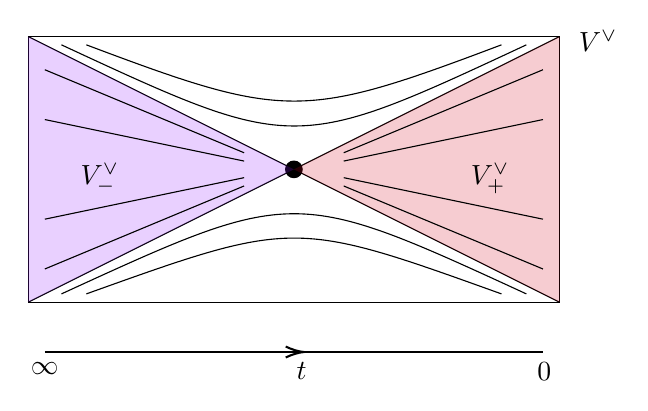
\begin{tikzpicture}[x=0.6pt,y=0.6pt,yscale=-1,xscale=1]
%uncomment if require: \path (0,300); %set diagram left start at 0, and has height of 300

%Shape: Rectangle [id:dp18937098784415363] 
\draw   (20,20) -- (340,20) -- (340,180) -- (20,180) -- cycle ;
%Straight Lines [id:da1318788053019485] 
\draw    (20,20) -- (340,180) ;
%Straight Lines [id:da9054914373607481] 
\draw    (20,180) -- (340,20) ;
%Straight Lines [id:da9510825035310609] 
\draw    (30,210) -- (330,210) ;
\draw [shift={(186,210)}, rotate = 180] [color={rgb, 255:red, 0; green, 0; blue, 0 }  ][line width=0.75]    (10.93,-3.29) .. controls (6.95,-1.4) and (3.31,-0.3) .. (0,0) .. controls (3.31,0.3) and (6.95,1.4) .. (10.93,3.29)   ;
%Shape: Circle [id:dp05608194391391974] 
\draw  [fill={rgb, 255:red, 0; green, 0; blue, 0 }  ,fill opacity=1 ] (175,100) .. controls (175,97.24) and (177.24,95) .. (180,95) .. controls (182.76,95) and (185,97.24) .. (185,100) .. controls (185,102.76) and (182.76,105) .. (180,105) .. controls (177.24,105) and (175,102.76) .. (175,100) -- cycle ;
%Shape: Triangle [id:dp24989332432828237] 
\draw  [draw opacity=0][fill={rgb, 255:red, 144; green, 19; blue, 254 }  ,fill opacity=0.2 ] (180,100) -- (20,180) -- (20,20) -- cycle ;
%Shape: Triangle [id:dp5377581483415403] 
\draw  [draw opacity=0][fill={rgb, 255:red, 208; green, 2; blue, 27 }  ,fill opacity=0.2 ] (180,100) -- (340,20) -- (340,180) -- cycle ;
%Straight Lines [id:da7000627750204172] 
\draw    (30,40) -- (150,90) ;
%Straight Lines [id:da5322630758087111] 
\draw    (30,70) -- (150,95) ;
%Straight Lines [id:da8248391946037721] 
\draw    (30,160) -- (150,110) ;
%Straight Lines [id:da2719071105268458] 
\draw    (30,130) -- (150,105) ;
%Straight Lines [id:da7756346880199279] 
\draw    (210,95) -- (330,70) ;
%Straight Lines [id:da21911398751314515] 
\draw    (210,90) -- (330,40) ;
%Straight Lines [id:da2981416153893458] 
\draw    (210,110) -- (330,160) ;
%Straight Lines [id:da27585222842907664] 
\draw    (210,105) -- (330,130) ;
%Curve Lines [id:da11209114331809367] 
\draw    (40,25) .. controls (180.33,90.17) and (180.33,90.17) .. (320,25) ;
%Curve Lines [id:da3693485194056053] 
\draw    (55,25) .. controls (175,70.17) and (185.33,70.17) .. (305,25) ;
%Curve Lines [id:da664510041065356] 
\draw    (40,175) .. controls (180,110.75) and (180,110.5) .. (320,175) ;
%Curve Lines [id:da46252259164860765] 
\draw    (55,175) .. controls (180,130.17) and (180.33,130.17) .. (305,175) ;

% Text Node
\draw (180,215) node [anchor=north west][inner sep=0.75pt]    {$t$};
% Text Node
\draw (20,215) node [anchor=north west][inner sep=0.75pt]    {$\infty $};
% Text Node
\draw (325,215) node [anchor=north west][inner sep=0.75pt]    {$0$};
% Text Node
\draw (50,95) node [anchor=north west][inner sep=0.75pt]    {$V_{-}^{\lor }$};
% Text Node
\draw (285,95) node [anchor=north west][inner sep=0.75pt]    {$V_{+}^{\lor }$};
% Text Node
\draw (350,15) node [anchor=north west][inner sep=0.75pt]    {$V^{\lor }$};


\end{tikzpicture}
	\end{figure}
\end{setup}


\begin{remark}\label{remark:homoteties}
	The restriction of the $\C^*$-action on $V^\vee$ defined in Set-up \ref{setup:atiyah} to $V_-^\vee$ (resp. $V_+^\vee$) coincides with $\C^*_h$-action on $V^\vee_-$ (resp. $V^\vee_+$) by homoteties.
\end{remark}

 The fixed point locus of this action on $V^\vee$ coincides with the origin. 
 We can consider the induced $\C^*$-action of the coordinate ring of $V^\vee$, namely $\C[V^\vee]=\C\left[y_0,\ldots,y_m,x_0,\ldots,x_l\right]$.
 The GIT-quotient $V^\vee\to V^\vee\git \C^*:=\Spec \C[V^\vee]^{\C^*}$ is the affine cone over the Segre embedding of $\P\left(V_-\right)\times \P\left(V_+\right) \simeq \P^m \times \P^l$, therefore singular at the origin of $V_-^\vee \otimes V_+^\vee$.

\begin{remark}\label{remark:cobordism}
	Under the notation of Definition \ref{def: cobordism}, we have that
	\begin{align*}
	&B_- \simeq V^\vee\setminus \left\{y_0=\ldots=y_m=0\right\},\\
	&B_+\simeq V^\vee\setminus \left\{x_0=\ldots=x_l=0\right\}.
	\end{align*}
	In particular $B_{\pm}$ are non-empty open subsets of stable points under the $\C^*$-action, therefore we have two geometric quotients $B_{\pm}\to B_{\pm}/\C^*$.
\end{remark}


\begin{lemma}\label{lemma:atiyahexceptionallocus}
	The geometric quotients $B_-/\C^*$ and $B_+/\C^*$ are birational, and the exceptional locus of the birational map $\psi: B_-/\C^*\dashrightarrow B_+/\C^*$ is $\P\left(V_-\right)$. In particular, $\psi$ is a small modification.
\end{lemma}

\begin{proof}
	Notice that $B_-/\C^*$ and $B_+/\C^*$ are birational since they contain the open subset $(B_-\cap B_+)/\C^*\neq \emptyset$ %= (V^\vee\setminus \left(\left\{y_0=\ldots=y_m=0\right\} \cup \left\{x_0=\ldots=x_l=0\right\} \right))/\C^*\neq \emptyset$.
	Let us study the exceptional locus of $\psi$. 
	It suffices to show that $V_-^\vee\setminus 0\subset B_-$ (then $\P\left(V_-\right)\subset B_-/\C^*$) and that $V_-^\vee\setminus 0\not\subset B_+$. 
	Let $p\in \P\left(V_-\right)$, and consider the associated line $\hat{p}$ in $V_-^\vee$ passing through the origin. Then $\hat{p}=\left(hv_-,0\right)$, for $h\in \C^*_h$ and $v_-\in V_-^\vee$. 
	For any point $q\in \hat{p} \setminus 0$ we have that that $\lim_{t\to \infty} t\cdot q$ does not exist, hence every point $q$ of $\hat{p}\setminus 0$ belongs to $B_-$. 
	By Remark \ref{remark:homoteties}, the restriction of the $\C^*$ on $V_-^\vee \setminus 0$ coincides with the action by homoteties, so we have that $p\in B_-/\C^*$. 
	On the other hand it is easy to see that $\lim_{t\to 0} t\cdot q$ exists, hence $q\notin B_+$.
	 Finally $\psi$ is a small modification since $\codim_{B_-/\C^*} \text{Exc}(\psi)\geq 2$. 
\end{proof}

\begin{remark}
	Let us recall that the example of Atiyah flip can be also easily described using toric geometry. In particular the birational map is induced by two different subdivisions of a cone. We refer to \cite[\S 3]{BR} for a detailed discussion from the toric point of view.
\end{remark}

\begin{corollary}
	The exceptional locus of $\psi^{-1}: B_+/\C^*\dashrightarrow B_-/\C^*$ is $\P(V_+)$.
\end{corollary}

\begin{remark}\label{remark:atiyahblowup}
	Let $\beta: W\to V^\vee\git \C^*$ be the blow-up of $V^\vee \git \C^*$ along the origin. Then the exceptional divisor is $\P(V_-)\times \P(V_+)$. 
\end{remark}

\begin{lemma}\label{lemma:atiyahfactorization}
	The blow-up $\beta: W\to V^\vee\git \C^*$ can be factorized through $b_{\pm}: W\to B_{\pm}/\C^*$ and the small contractions $s_{\pm}: B_{\pm}/\C^*\to V^\vee\git \C^*$ with exceptional loci $\P(V_{\pm})$. 
\end{lemma}

\begin{proof}
	There exist two natural birational morphisms $s_{\pm}: B_{\pm}/\C^*\to V^\vee\git \C^*$, isomorphisms over the set of points which are semistable but not stable. From this it follows that $\Exc(s_{\pm})=\P(V_{\pm})$. Since they have codimension greater than two, we conclude $s_{\pm}$ are small contractions. 
	Moreover, since $W$ is birational to $V^\vee\git \C^*$, which is birational to $B_{\pm}/\C^*$, we conclude there exist birational maps $b_{\pm}: W\dashrightarrow  B_{\pm}/\C^*$, defined over $W\setminus (\P(V_-)\times \P(V_+))$. Since the exceptional locus has codimension one, $b_{\pm}$ are morphisms.	
	Let us prove that $b_{\pm}\circ s_{\pm}=\beta$. For sake of simplicity, let us consider $b_-\circ s_-$. It is immediate to notice that $b_-^{-1}(s_-^{-1}(0))=b_-^{-1}(\P(V_-))=\P(V_-)\times \P(V_+) =\beta^{-1}(0)$. 
\end{proof}



We summarize the above construction by means of the diagram

%\begin{center}
\[
\xymatrix{ & W \ar[ld]_{b_-} \ar[rd]^{b_+} \ar[dd]^<<<<<<\beta & \\ B_-/\C^* \ar@{-->}[rr]^<<<<<<\psi \ar[rd]_{s_-} && B_+/\C^* \ar[ld]^{s_+} \\ & V^\vee \git \C^* & }
\]


and its restriction to the exceptional loci:
\[
\xymatrix{ & \P\left(V_-\right) \times \P\left(V_+\right) \ar[ld]_{b_-} \ar[rd]^{b_+}  & \\ \P\left(V_-\right) \ar[rd]_{s_-} && \P\left(V_+\right) \ar[ld]^{s_+} \\ & 0 &}
\]


\begin{theorem}
	The birational map $\psi:B_-/\C^*\dashrightarrow B_+/\C^*$ is a rooftop flip modeled by $\P(V_-)\times \P(V_+)$.
\end{theorem}

\begin{proof}
	We verify that each condition of Definition \ref{def:Dflips} is satisfied.
	For $(1)$, Using Lemma \ref{lemma:atiyahexceptionallocus}, the birational map $\psi: B_-/\C^*\dashrightarrow B_+/\C^*$ is a small modification, the exceptional loci of $s_{\pm}: B_{\pm}/\C^*\to \hat{X}\git \C^*$ are $\P(V_{\pm})$ and the restriction $s_{\pm}|_{\P(V_{\pm})}: \P(V_{\pm}) \to 0$ are obviously $\P(V_{\pm})$-bundles. 
	Let us prove verify $(2)$: if we consider the resolution $b_{\pm}: W\to B_{\pm}/\C^*$ we have that $\P(V_-)\times \P(V_+)=b^{-1}_{\pm}(\P(V_{\pm}))$ is a divisor, and $\P(V_-)\times \P(V_+)\to \P(V_{\pm})$ defines two projective bundle structures.
	Finally, we consider $(3)$: In this case $Z_0$ is the origin, and we know that $s^{-1}_{\pm}(0)\simeq \P(V_{\pm})$. Moreover $(b_{\pm}^{-1}\circ s_{\pm}^{-1})(0)\simeq \P(V_-)\times \P(V_+)$, hence we conclude.
\end{proof}

\begin{corollary}
	The geometric quotients $B_{\pm} /\C^*$ are smooth, and the rooftop flip $\psi: B_-/\C^*\dashrightarrow B_+/\C^*$ is in particular a small $\Q$-factorial modification.
\end{corollary}

\begin{proof}
	Since the non-empty open subset $B_{\pm}$ are smooth, and $\C^*$ acts freely on them, using \cite[Corollary p.199]{MFK} we obtain that $B_{\pm}$ are $\C^*$-principal bundles over $B_{\pm}/\C^*$, hence they are smooth. 
\end{proof}






